\documentclass[]{article}
\usepackage[a4paper, total={6in, 8in}]{geometry}
\usepackage{pdflscape}
\usepackage{booktabs}
\usepackage{multicol}
\usepackage{mathtools, amssymb, amsmath}
\usepackage{afterpage}
\usepackage[
  sorting=nty,
  backend=bibtex,
  giveninits=true,
  style=authoryear-comp,
  natbib=true,
  maxcitenames=2,
  useprefix=true,
  uniquename=init,
]{biblatex}
\bibliography{bibliography}

\newcommand{\todo}[1]{{\color{red}[\textit{TODO: #1}]}}
\newcommand{\todonocomment}[1]{{\color{red}[\textit{#1}]}}

\makeatletter
\newcommand{\citetnl}[1]{%
  \@firstofone{\citet{#1}}}
\makeatother

\usepackage{tikz}
\usetikzlibrary{calc}
\usetikzlibrary{shapes.geometric, arrows, fit}

\tikzstyle{process} = [rectangle, 
minimum width=12cm, 
minimum height=1cm, 
text width=11cm, 
draw=black, 
fill=white,
rounded corners]

\tikzstyle{subprocess} = [rectangle, 
minimum width=5cm, 
minimum height=0.6cm, 
text centered, 
text width=5cm, 
draw=black, 
fill=white]

\tikzstyle{lsnode} = [rectangle, 
minimum width=2cm, 
minimum height=0.6cm, 
text centered, 
text width=2cm, 
draw=black, 
fill=white]

\tikzstyle{arrow} = [thick,->,>=stealth]
\tikzstyle{dashedarrow} = [dashed,->,>=stealth]

\title{Integrated Vehicle and Crew Scheduling for Electric Buses with Realistic Charging Behavior}
\date{July 2025}
\author{Thomas van der Plas, Han Hoogeveen, Philip de Bruin}
\begin{document}
\maketitle

\section{Introduction}
Electric vehicles are beginning to make up large portions of the fleet for public transport providers. In The Netherlands for example, approximately 21\% of all registered buses utilize an electric drivetrain, as reported by the \citet{RDW}. To comply with strict Dutch and the European \citet{europaRegulation20181999} on climate and sustainability, this proportion must increase substantially; from 2025 onward, the procurement of new buses powered by non-renewable energy sources will no longer be permitted, with the objective that by 2030, all public transport buses operate with zero emissions. Individual line operators such as \citet{qbuzzQbuzz} are therefore rapidly replacing their remaining buses that use fossil fuels, resulting in primarily electric-powered fleets. \\
Effective use of these new electric vehicles is however more challenging than that of a combustion based fleet. One of the logistical steps in which this is most apparent is that of vehicle scheduling. The Vehicle Scheduling Problem (VSP) aims to assign vehicles such that a set of trips is covered; in the case of buses, these trips are defined by the timetables for individual lines. A typical solution to this problem comes in the form of a collection of vehicle tasks, each of which can be seen as a schedule that an individual bus will follow throughout the day. It may start at a bus storage facility (more commonly called a depot), then perform one or more trips, before finally returning to the depot. In order to string multiple trips together, a bus must make an empty travel from the ending location of one trip to the starting location of the next. These empty travels, often called deadheads, are the main focus when determining the overall costs of a collection of vehicle tasks. There is ample choice as to which deadheads can be driven, as in theory the deadhead between each pair of compatible trips can be included during the creation of a vehicle task. It is therefore necessary to determine which of these deadheads are required in order to drive all trips while minimizing costs. \\
In the VSP and its variants, a commonly made assumption is that a vehicle can travel an entire day without having to refuel. With electric vehicles, this assumption is often not valid: recharging throughout the day is required as the range of an electric vehicle is limited. Additionally, recharging takes a long time when compared to the refueling of a combustion vehicle: refueling can be done in a matter of minutes, whereas recharging may take multiple hours for a full charge. The electrification of fleets therefore requires the VSP to be adapted to include maximum range constraints, as well charging possibilities within a vehicle task. This extended version of the problem, often referred to as the Electric Vehicle Scheduling Problem (E-VSP), is significantly harder than its non-electric counterpart; the VSP with a single depot can be solved in polynomial time, whereas the E-VSP is NP-Hard as shown by \citet{Bunte2009} and \citet{Sassi2014} respectively. \\
In addition to this added computational complexity in the E-VSP, other logistical planning steps are effected as well. The Crew Scheduling Problem (CSP) is commonly the step that follows vehicle scheduling. Here, schedules are made for individual crew members such that the planned vehicles always have a driver associated with them. As crew members are subject to labor regulations, additional constraints are now added when compared to vehicle scheduling such as maximum driving time and required breaks. The CSP is also NP-Hard, as shown by \citet{Fischetti1989}.\\
Costs in this step often exceed those associated with the vehicles themselves, with a recent estimate by \citet{Perumal2019Crew} putting crew member costs at around 60\% of all operational costs. Optimal solutions for the CSP are however directly influenced by the selected vehicle tasks; they determine where and at what time handovers of vehicles are possible between crew members. Sequentially minimizing costs in the VSP and CSP may therefore not result in a solution with overall lowest costs, as the solution to the CSP may be improved greatly by incurring higher costs in the VSP. This was already pointed out in the 1980s by \citet{Bodin1983}, who instead advocated for an integrated approach; here, the costs of the VSP and CSP are minimized simultaneously, resulting in the Vehicle and Crew Scheduling Problem (VCSP). \\
A lot of work has already been done on the VSP, CSP and VCSP. Both the sequential and integrated approach have been extensively studied since the 1980s, as shown by reviews such as \citet{Ibarra-Rojas2015} and \citet{Ge2024}. As mentioned before however, the introduction of electric vehicles has introduced significant constraints on recharging times and vehicle ranges, invalidating the critical assumption in many of these works that a vehicle was able to drive an entire day without being refueled. As a response to this, the E-VSP has also been the focus of many studies going back to around 2014. We refer the reader to a survey by \citet{Perumal2022LitRev} for a detailed overview of recent progress. \\
The integrated VCSP with electric vehicles (E-VCSP) has seen less attention; to the best of our knowledge, only 5 works consider this problem. In these, simplifying assumptions are made about battery charging behavior which might limit real world applicability or accurate modeling of costs. In this work, our aim is therefore to introduce an integrated E-VCSP model which incorporates more realistic behavior for battery charging. \\
The rest of this work is organized as follows. In Section 2, we will give more background information on the E-VCSP and provide a formal problem definition. In Section 3, we review literature related to the E-VCSP and identify gaps in the current research. \dots. An overview of nomenclature and abbreviations used throughout this work has been included in Table \ref{tab:nomenclature}.

\begin{table}
  \centering
  \begin{tabular}{ll}
    \toprule
    \multicolumn{1}{l}{\textbf{Abbreviation}} & \multicolumn{1}{l}{\textbf{Definition}}               \\
    \cmidrule(lr){1-1}\cmidrule(lr){2-2}
    ALNS                                      & Adaptive Large Neighborhood Search                    \\
    B\&P                                      & Branch-and-Price                                      \\
    CG                                        & Column Generation                                     \\
    CP                                        & Constraint Programming                                \\
    CSP                                       & Crew Scheduling Problem                               \\
    E-\dots                                   & Problem \dots with electric vehicles                  \\
    LNS                                       & Large Neighborhood Search                             \\
    LS                                        & Local Search                                          \\
    MDVSP                                     & Multi Depot Vehicle Scheduling Problem                \\
    MIP                                       & Mixed Integer Program                                 \\
    SAA                                       & Simulated Annealing Algorithm                         \\
    SDVSP                                     & Single Depot Vehicle Scheduling Problem               \\
    SoC                                       & State of Charge                                       \\
    TCO                                       & Total Cost of Ownership                               \\
    ToU                                       & Time of Use                                           \\
    TVSP                                      & Integrated Timetabling and Vehicle Scheduling Problem \\
    VCSP                                      & Integrated Vehicle and Crew Scheduling Problem        \\
    VSP                                       & Vehicle Scheduling Problem                            \\
    \bottomrule
  \end{tabular}
  \label{tab:nomenclature}
  \caption{Nomenclature used in this work}
\end{table}

\section{Problem definition}
\label{sec:problem_def}
In this section, we give a definition of the integrated Electric Vehicle and Crew Scheduling Problem (E-VCSP). In order to do so, we will first give a global overview of the problem at hand. Afterwards, we discuss the data which is given, before finally formalizing our the resulting problem.

\begin{figure}
  \centering
  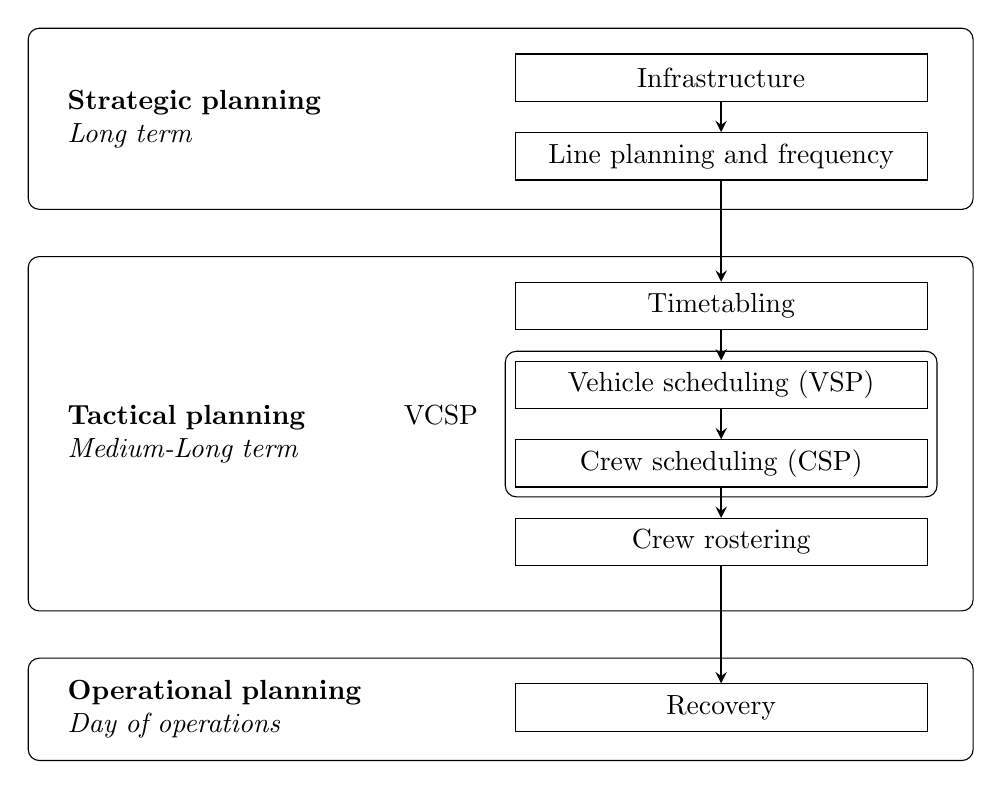
\begin{tikzpicture}[node distance=2cm]
    \node (strategic) [process, minimum height=2.3cm] {\textbf{Strategic planning}\\\textit{Long term}};
    \node at (strategic.base) (infra) [subprocess, xshift=2.8cm, yshift=0.4cm] {Infrastructure};
    \node at (strategic.base) (line) [subprocess, below of=infra, yshift=1cm] {Line planning and frequency};

    \node (tactical) [process, minimum height=4.5cm, below of=strategic, yshift=-2cm] {\textbf{Tactical planning}\\\textit{Medium-Long term}};
    \node at (tactical.base) (timetable) [subprocess, xshift=2.8cm, yshift=1.5cm] {Timetabling};
    \node at (tactical.base) (vehicle) [subprocess, below of=timetable, yshift=1cm] {Vehicle scheduling (VSP)};
    \node at (tactical.base) (crew) [subprocess, below of=vehicle, yshift=1cm] {Crew scheduling (CSP)};
    \node at (tactical.base) (VCSP) [rounded corners, draw=black, fit=(vehicle) (crew), align=left] {\hspace{-4em}VCSP};
    \node at (tactical.base) (rostering) [subprocess, below of=crew, yshift=1cm] {Crew rostering};

    \node (operational) [process, minimum height=1.3cm, below of=tactical, yshift=-1.5cm] {\textbf{Operational planning}\\\textit{Day of operations}};
    \node at (operational.base) (recovery) [subprocess, xshift=2.8cm, yshift=-0.1cm] {Recovery};

    \draw [arrow] (infra) -- (line);
    \draw [arrow] (line) -- (timetable);
    \draw [arrow] (timetable) -- (vehicle);
    \draw [arrow] (vehicle) -- (crew);
    \draw [arrow] (crew) -- (rostering);
    \draw [arrow] (rostering) -- (recovery);
  \end{tikzpicture}
  \caption{A general overview of the public transport planning process, based on \citet{Ceder1986, Ibarra-Rojas2015, Perumal2022LitRev}.}
  \label{fig:planning-overview}
\end{figure}

\subsection{Overview}
The E-VCSP is part of the planning process used in bus public transit, as can be seen in Figure \ref{fig:planning-overview}. It comes directly after the timetabling step, in which trips are defined for each line according to passenger demand. Each individual timetabled trip represents a bus traveling along a line at a specified time. Oftentimes, these trips are scheduled regularly throughout the day from the start to the end of a line, however irregular schedules and partial travels are also possible. \\
With these trips being laid out, we now need to determine how they will be driven. Individual trips often have lengths of around 0.5-2 hours, therefore making it possible to perform multiple trips with a single vehicle and driver in a day. In order to perform a trip, a vehicle must travel to its starting location before driving it; this travel is called a deadhead. Deadheads occur between trips and between a trip and a depot. During a deadhead, the vehicle itself is empty except for the driver. It is therefore beneficial to minimize the total amount of time that vehicles and crew members spend driving deadheads, as costs incurred during this time do not have any direct benefit to passengers. \\
When considering electric vehicles, the time between trips is not only used for driving deadheads. As electric vehicles generally have small ranges and long recharging times, this downtime can also be used in order to recharge the vehicle. Often, recharging stations will be available at the depot, however additional recharging stations may also be present at the starting or ending locations of trips (also called the terminal trip stops). Charging locations in the middle of a trip are generally not present. \\
Recharging a vehicle at a certain location follows a given charging curve; this curve defines the charging power when a vehicle is at a certain state of charge. This curve is generally split into two phases: from 0 to around 80\%, in which the charging rate is roughly constant, and from 80 to 100\%, where it slows significantly. These phases often take similar amounts of time. \\
Performing a full charge of a vehicle may take on the order of hours, even when fast-charging infrastructure is available; the resulting vehicle downtime therefore necessitates careful planning of crew schedules. Crew members must follow local labor regulations, which often consist of maximum driving times throughout the day and required breaks. Combining these breaks with charging time for the vehicle can therefore be beneficial. Additionally, crew members can use multiple vehicles throughout the day, further reducing crew downtime if a certain vehicle is required to wait for a trip. \\
Vehicle handovers are often only possible at a predetermined set of locations; these relief points have waiting areas or break rooms connected to them, providing a place for a crew member to stay before entering their next vehicle. This implies that handovers cannot always occur on a trip by trip basis; the schedules of vehicles and drivers can be broken up into multiple blocks, each of which starts and ends at a relief point. The resulting blocks must be driven by a single driver, as handovers during the block are not possible. \\
Lastly, drivers may sometimes travel between different locations by means other than driving a vehicle. An example of this may be when locations are geographically close, allowing a driver to walk between them if required. This provides additional flexibility in handover procedures, and allows for a central break location to be present when multiple stops are close to one another. \\
Overall, the goal is to find a set of feasible vehicle and crew schedules that minimizes costs. In this, vehicle schedules must ensure that each trip is driven while minimizing deadhead and charging costs. These schedules must also ensure that enough charging takes place such that the vehicle state of charge is within acceptable levels. Crew schedules, on the other hand, must ensure that each driven block is covered. While doing so, local labor regulations must be taken into account.

\begin{table}[h]
  \centering
  \begin{tabular}{ll}
    \toprule
    \multicolumn{1}{l}{\textbf{Notation}} & \multicolumn{1}{l}{\textbf{Definition}}               \\
    \cmidrule(lr){1-1}\cmidrule(lr){2-2}
    \multicolumn{2}{l}{\textit{Given}} \\
    $\mathcal{D}$ & The depot \\ 
    $t \in \mathcal{T}$ & Set of all trips, $t$ a single trip \\
    $dh \in \mathcal{DH}$ & Set of all feasible deadheads, $dh$ a single deadhead \\ 
    $b \in B$ & Set of all blocks, $b$ a single block \\
    $v \in V$ & Set of all vehicle tasks, $v$ single vehicle task \\
    $c \in C$ & Set of all crew tasks, $c$ single crew task \\
    $d_\chi$ & Amount of charge used driving a trip/deadhead \\
    $u_{dh,\sigma}$ & Max. charge gained in deadhead $dh$ with starting SoC $\sigma$ \\
    $\sigma_{start}$ & SoC at beginning of block/task \\
    $\sigma_{min}$ & Minimum SoC of vehicle \\
    $\sigma_{max}$ & Maximum SoC of vehicle \\ 
    $k_{i,t}$ & Binary constant, vehicle task $v_i$ covers trip $t$ \\ 
    $l_{i,b}$ & Binary constant, vehicle task $v_i$ uses block $b$ \\ 
    $m_{j,b}$ & Binary constant, crew task $c_j$ uses block $b$ \\ 
    \addlinespace[0.6em]
    \multicolumn{2}{l}{\textit{Decision variables}} \\
    $x_{i} \in \{ 0, 1 \}$ & Usage of vehicle task $v_i$  \\ 
    $y_{j} \in \{ 0, 1 \}$ & Usage of crew task $c_j$ \\ 
    \addlinespace[0.6em]
    \multicolumn{2}{l}{\textit{Helper functions}} \\
    $b(v) \subseteq B$ & Set of blocks covered by $v$ \\ 
    $cost(\chi) \in \mathbb{R}^+$ & Cost of task $\chi$ \\ 
    \addlinespace[0.2em]
    \bottomrule
  \end{tabular}
  \label{tab:notation}
  \caption{Notation used for formal problem description, where $\chi$ is used as a placeholder when multiple argument types can be applied.}
\end{table}

\subsection{Formal definition}
We will now formally define the E-VCSP. In this, we will consider the variant with a single depot, single vehicle type and charging stations without capacity limitations. Additionally, partial and non-linear charging are considered. A summary of the notation used has been provided in Table \ref{tab:notation}. \\
Given timetables for each of the considered lines, let $\mathcal{T}$ be the set of trips that they define. Additionally, let $\mathcal{DH}$ be the set of deadheads that represent either a travel to or from the depot $\mathcal{D}$, or a travel between trips in $\mathcal{T}$. In this, only deadheads are present which can feasibly be driven; that is, the travel time of the deadhead must be less than the time between its departure and the start of a target trip. Note that deadheads including a depot as either the origin or target are always considered to be time-feasible. \\ 
Next, let us define our battery behavior. For each trip $t$ and deadhead $dh$, let $d_t$ and $d_{dh}$ respectively indicate the amount of charge that is used during its travel. Additionally, let $u_{dh,\sigma}$ indicate the maximum amount of charge that can be gained during a deadhead if a vehicle starts the deadhead at a State of Charge (SoC) of $\sigma$; in this, let charging at any possible given charging location be considered. Depending on available charging infrastructure, this may imply that a deadhead is not driven directly, instead making a time-feasible detour via a charging location which provides the fastest charging capabilities. SoC gained at a location depends on given (possibly non-linear) charging curves for the vehicle, allowing for different amounts of charge to be achieved in the same time span depending on the initial SoC. Note that when discrete SoC values are used, all values of $u_{dh,\sigma}$ can be precomputed. \\
Lastly, let us define relief points. A subset of the terminal locations of trips may serve as relief points; these locations are the only ones at which a handover or break for a crew member can take place. Using these relief points, we can now start formally defining our schedules.\\
Let a \textit{block} be a sequence of trips and/or deadheads that can be driven sequentially, in which only the first and last location in the sequence are relief points. This implies that a block must be driven by a single driver, as there is no opportunity to hand over the vehicle to another driver during the block itself. In order to be feasible, the block must match the following requirements: 
\begin{itemize}
  \item A block consists of at least one trip or deadhead.
  \item Only the first and last location visited in the block are relief points.
  \item If there is an element in the block directly following a trip, this must be a deadhead originating from that trip.
  \item If there is an element in the block directly following a deadhead, this must be the target trip of the deadhead.
  \item For each deadhead $dh$ driven, the vehicle must charge with some value $\alpha \cdot u_{dh,\sigma}$, where $0 \leq \alpha \leq 1$ represents a fraction of the maximal charge gained. 
  \item Given an SoC $\sigma_{start}$ at the beginning of the block, the SoC of the vehicle should remain within the range $[ \sigma_{min}, \sigma_{max} ]$ throughout the block.
\end{itemize}
Let the set of all feasible blocks be $B$. A schedule for a vehicle throughout the day can now be constructed as a sequence of blocks. Let us refer to such a schedule as a \textit{vehicle task}. In order for a vehicle task to be feasible, the following conditions need to be met:
\begin{itemize}
  \item A vehicle task consists of one or more blocks. 
  \item Sequential pairs of blocks must be compatible; that is, for each sequential pair of blocks $b$ and $b'$, $b$ must either end in a deadhead whose target is the starting trip of $b'$, or $b$ must end in a trip which is the origin of the starting deadhead of $b'$.
  \item The task must start and end at the depot. 
  \item Given an SoC $\sigma_{start}$ at the beginning of the task, the SoC of the vehicle should always remain within $[ \sigma_{min}, \sigma_{max} ]$ during all blocks.
\end{itemize}
Let the set of all feasible vehicle tasks be $V$. For a vehicle task $v$, let us define its cost as being $cost(v)$; let this be some combination of fixed and variable costs based on the trips and deadheads driven within the task. \\
Next, let us consider crew tasks. Crew members are bound by labor regulations; in most cases, this means that we will need to include break time in a crew schedule. Additionally, idle time at a handover location may be required in order to wait for an arriving vehicle. Lastly, crew members may travel to different locations without driving a vehicle. A crew task will therefore consist of a sequence of subtasks which may contain blocks to be driven, idle/break times, and travels to other locations. Exact feasibility constraints for crew tasks will differ per country and region, however we base the following constraints on a simplified version of the Dutch labor regulations: 
\begin{itemize}
  \item The crew task consists of one or more blocks, travels or break/idle times.
  \item Sequential pairs of blocks must be compatible. That is, for each sequential pair of blocks $b$ and $b'$, the location at the end of $b$ must be the same as the start of $b'$. Additionally, the ending time of $b$ must be equal to the starting time of $b'$. 
  \item The crew task must start and end at the depot.
  \item The crew task may have a duty length of at most 9 hours 
  \item A crew member may drive for at most 4 hours without a break.
  \item For tasks between 4 and 5.5 hours, at least one break of 15 minutes must be included. 
  \item For tasks longer than 5.5 hours, at least 40 minutes of break time must be included. All breaks must be longer than 15 minutes, and one break must be at least 20 minutes.
  \item For tasks starting after 15:00, at least one break between 16:30 and 20:30 of at least 20 minutes must be included. 
\end{itemize}
Of these, the first three constraints will be applicable regardless of local labor regulations. Let the set of all feasible crew tasks be $C$. For a crew task $c$, let us define its cost as being $cost(c)$; let this be some combination of fixed and variable costs based based on duty and break length. \\\\
Using the definitions of the blocks $B$, vehicle tasks $V$ and crew tasks $C$, we can formulate a linear program to describe our integrated problem. In this, let $x_i$ and $y_j$ be binary variables indicating the usage of $v_i \in V$ and $c_j \in C$ respectively. Additionally, let $k_{i,t} \in \{ 0, 1 \}$ indicate that $v_i$ covers trip $t \in \mathcal{T}$, let $l_{i,b}$ indicate that $v_i$ contains block $b \in B$, and let with $m_{j,b} \in \{ 0, 1 \} $ indicate that $c_j$ includes block $b \in B$. Our cost minimization can then be formulated as follows:
\begin{align}
\min \quad
& \sum_{1 \leq i \leq |V|} x_{i} \cdot cost(v_i) + \sum_{1 \leq j \leq |C|} y_{j} \cdot cost(c_j)  
\end{align}
Subject to:
\begin{align}
\sum_{1 \leq i \leq |V|} x_{i}a_{it} &= 1 && \forall t = 1,\:\dots,\:|T| \label{form:all-trips-covered} \\
\sum_{1 \leq i \leq |V|}x_i l_{i,b}  &= \sum_{1 \leq j \leq |C|}y_j m_{j,b}  && \forall b \in B \label{form:all-blocks-covered} \\
x_{i} &\in \{ 0, 1 \} && \forall i = 1,\:\dots,\:|V| \\
y_{j} &\in \{ 0, 1 \} && \forall j = 1,\:\dots,\:|C|
\end{align}
Here, constraint (\ref{form:all-trips-covered}) ensures that all trips are covered by a vehicle, and constraint (\ref{form:all-blocks-covered}) ensures that for each block, the number of assigned drivers is equal to the number of assigned vehicles. This integrated formulation minimizes the costs for both vehicle and crew tasks simultaneously. For comparison, when the E-VSP and CSP are solved sequentially, the formulation becomes the following. First, vehicle tasks are selected such that their costs are minimized:
\begin{align}
\min \quad
& \sum_{1 \leq i \leq |V|} x_{i} \cdot cost(v_i)
\end{align}
Subject to:
\begin{align}
\sum_{1 \leq i \leq |V|} x_{i}a_{it} &= 1 && \forall t = 1,\:\dots,\:|\mathcal{T}| \label{form:all-trips-covered-seq} \\
x_{i} &\in \{ 0, 1 \} && \forall i = 1,\:\dots,\:|V|
\end{align}
Here, constraint (\ref{form:all-trips-covered-seq}) once again ensures that all trips are covered by a vehicle task. Once the vehicle tasks are selected, we can use them to derive the set of blocks that are driven. Let $b(v) \subseteq B$ represent the set of blocks driven by a vehicle task $v$. The overall set of blocks driven is then $B' = \bigcup_{v_i \in V, x_i = 1}b(v_i)$, and let the crew tasks for which all used blocks appear in $B'$ be $C'$. Note that in our construction of $B'$, each block is present at most once due to the fact that all trips are covered exactly once in our E-VSP formulation. \\
Using this, our formulation for crew tasks becomes the following:
\begin{align}
\min \quad
& \sum_{1 \leq j \leq |C'|} y_{j} \cdot cost(c_j)  
\end{align}
Subject to:
\begin{align}
\sum_{1 \leq j \leq |C'|} y_j m_{j,b} &= 1  && \forall b \in B' \label{form:all-blocks-covered-seq} \\
y_{j} &\in \{ 0, 1 \} && \forall j = 1,\:\dots,\:|C'|
\end{align}
Here, we now consider a greatly reduced number of available blocks and crew tasks, resulting in a formulation with significantly less rows and columns than the equivalent integrated formulation.

\section{Related work}
In this section, we discuss work related to our research into the E-VCSP. A summary of how batteries and charging behavior are modeled in the discussed works has been included in Table \ref{tab:eVCSP-lit}.

\afterpage{
  \clearpage
  \begin{landscape}
  \null
  \vfill
  \begin{table}[h!]
    \centering
    \begin{tabular}{llllllll}
      \toprule
                                        & Model   & ToU & SoC & Nonlinear Ch. & Partial Ch. & Ch. Location & Degradation \\
      \cmidrule(lr){2-8}
      \citet{Li2014}               & E-VSP   & No  & D   & No            & No          & D            & No          \\
      \Citet{vanKootenNiekerk2017} & E-VSP   & Yes & C/D & Yes           & Yes         & D/T          & Yes         \\
      \citet{Olsen2020}            & E-VSP   & No  & C   & Yes           & Yes         & D/T          & No          \\
      \citet{Zhang2021}            & E-VSP   & No  & C/D & Yes           & Yes         & D            & Yes         \\
      \citet{Parmentier2023}       & E-VSP   & No  & C   & Yes           & Yes         & D/T          & No          \\
      % \citet{Pulyassary2024}       & E-VSP   & No  & C/D & Yes           & Yes         & T            & No          \\
      \Citet{deVos2024}            & E-VSP   & No  & D   & Yes           & Yes         & D/T          & No          \\
      \addlinespace[0.4em]
      \citet{Perumal2021}          & E-VCSP  & No  & C   & No            & No          & D            & No          \\
      \citet{Wang2022}             & E-VCSP  & Yes & C   & No            & Yes         & D            & No          \\
      \citet{Sistig2023}           & E-VCSP  & No  & C   & No            & Yes         & D/T          & No          \\
      \citet{Shen2023}             & E-VCSP  & No  & C   & No            & Yes          & D/T          & No          \\
      \citet{Cong2024}             & E-VCSP  & Yes & C   & No            & Yes         & D            & No          \\
      \addlinespace[0.4em]
      \citet{Ham2021}              & E-VRPTW & Yes & C   & No            & Yes         & D            & No          \\
      \citet{Stadnichuk2024}       & E-TVSP  & No  & C   & No            & Yes         & D/T          & No          \\
      \bottomrule
    \end{tabular}
    \caption{A brief overview of battery modeling in E-VCSP related literature. SoC modeled as (D)iscrete or (C)ontinuous variable, Charge locations at (D)epot or (T)erminal trip stops, Degradation of battery in cost function}
    \label{tab:eVCSP-lit}
  \end{table}
  \vfill
  \end{landscape}
  \clearpage
}

\subsection{(E-)VSP}
Before considering previous work on the E-VSP, we first cover the most basic form of vehicle scheduling: that which only considers a single depot, single vehicle type and unlimited vehicle ranges. This problem, often referred to as the Single Depot Vehicle Scheduling Problem (SDVSP), forms the underlying basis of both the multi-depot and electric vehicle extensions that we consider later. We therefore give a brief summary of one the most common models and solution methods used for the SDVSP, thereby having a baseline to which we can compare extensions. For a more comprehensive overview on different models used for the SDVSP and Multi-Depot VSP (MDVSP), we refer the reader to a review by \citet{Bunte2009}. \\
In order to find a solution the SDVSP, the problem can be transformed into one of finding a min-cost max-flow in a graph. The graph can be constructed as follows: For all trips $\mathcal{T}$, add a pair of nodes representing the start and end of the trip respectively. Add an arc from the start of each trip to its end with capacity 1 and cost equal to that of driving the trip. Next, connect the end of each trip $t$ to the start of each trip $t'$ for which the deadhead between the two is feasible; that is, there is enough time to drive the deadhead from $t$ to $t'$ before the scheduled starting time of $t'$. Let each of these arcs have a capacity 1 and a cost equal to that of driving the deadhead from $t$ to $t'$. Lastly, let us introduce a pair of nodes representing the depot at the start and end of the day respectively. Connect the depot start node to the start of each trip, and do the same for the depot end node and the end of each trip. For each of these arcs, let the capacity once more be 1 and let the cost be equal to that of driving of the deadhead between the depot and trip. Fixed vehicle costs can be represented by adding costs to the arcs leaving the depot. \\
We can now find the min-cost max-flow on this graph; in this, let the depot start node be the source, and let de depot end node be the sink. Due to our construction, all trips must be covered by exactly 1 flow, resulting in flow paths which we can directly use as vehicle tasks due to the assumption that our vehicles have infinite range. It is therefore also shown that the SDVSP can be solved in polynomial time, as polynomial time min-cost max-flow algorithms exist and the graph elements are of size $|V| = O(|\mathcal{T}|)$ and $|A| = O(|\mathcal{T}|^2)$.\\ 
Two common extensions to the problem make it NP-Hard: the inclusion of multiple vehicle types, as well the use of multiple depots under the assumption that vehicles must return to their depot of origin. Both of these extensions are also discussed in \citet{Bunte2009}. The modification to the SDVSP flow network is the same in either case: an additional source/sink pair can be added for each new depot or vehicle type, and connected to the trips in the same way as the original depot. The problem then turns into into an integral multi-commodity flow, which has been shown to be NP-Hard by \citet{Even1975}. \\
The introduction of any resource constraints within the VSP has also been shown to be NP-Hard by \citet{Bodin1983}. The E-VSP specifically deals with constraints on the driving range of vehicles, thereby making it closely related to the vehicle scheduling problem with route time constraints (VSP-RTC) as described by \citet{Haghani2002}. The key difference between these two problems is that the E-VSP allows for (partial) recharging of a vehicle throughout the operating period, whereas the VSP-RTC assumes a fixed maximum travel time for the vehicle within the given period. The E-VSP has been shown to be NP-Hard by \citet{Sassi2014}. \\\\
\citet{Li2014} is one of the first to consider a solution method for the E-VSP. They consider a single-depot case with a single vehicle type, in which the assumption is made that full recharging (or battery swaps) can be performed in a fixed 5-minute time window. The model is based on the traditional SDVSP network, with the inclusion of driving time constraints for the vehicle tasks. Additionally, time-discretized nodes are added to represent capacitated battery charging/swap stations. Connections are made from the trip nodes to the charging nodes when a travel between the two is feasible, allowing for a vehicle to perform one or more charging action during its task. By using discretized charging nodes, charging station capacity is enforced with the use of flow constraints. For smaller instances, the model can be solved to optimality using column generation and branch-and-price (B\&P). For larger instances, an alternate approach using truncated column generation followed by a local search to find a local optimum is used instead. The proposed methods are tested on trips in the San Francisco Bay Area, with a maximum instance size of 242 trips. These tests resulted in optimality gaps of $<5\%$ for buses able to drive 150km, and between 7-15\%  for a range of 120km depending on the instance. \\
\Citet{vanKootenNiekerk2017} introduce two models which aim to solve the single depot E-VSP while taking into account time dependent energy prices (ToU pricing), nonlinear charging times and battery degradation due to depth of discharge. The first model extends the traditional SDVSP model by discretizing the depot nodes over time, and adding a continuous variable to each trip node representing the vehicle SoC at its start. This only allows for the formulation that uses linear charging curves, and does not incorporate degradation or ToU. The second model does allow for the extra inclusions, achieving this by now additionally discretizing both depot and trip nodes for individual starting SoC values. Charge-feasibility of deadheads can then be considered during graph construction, only adding arcs between nodes when the SoC difference between them can be achieved through driving and charging during the deadhead. The second model is solved using CG and lagrangian relaxation, resulting in an optimist solution. Tests are performed using data provided by Belgian bus company De Lijn in the city Leuven, using a total of 543 trips. They show that the second model can be solved in a considerably shorter time frame for large instances with similar results to the first. \\  
\citet{Olsen2020} consider a multi-depot E-VSP, in which they model the nonlinear phase of charging as an exponential function. In order to solve, they implement a greedy heuristic to construct vehicle tasks. Their primary focus is comparing (piecewise) linear approximations for the second phase of charging with an exponential function based approximation. They conclude that SoC and required charging times are more comparable to real life behavior when using the exponential function. \\
\citet{Zhang2021} consider an E-VSP variant with a single depot, capacitated charging infrastructure, non-linear charging behavior and battery degradation. They model this by combining elements from \citet{Li2014} and \citet{vanKootenNiekerk2017}, resulting in a network which has time and charge discretized depot, trip and charging station nodes; arcs between these are again only present if the deadhead is both time and charge-feasible. Solutions are found using a combination of CG and B\&P, and tests are performed on both randomly generated instances as well as 6 not yet electrified lines with up to 160 and 197 trips respectively. \\
\citet{Parmentier2023} consider a scalable approach to the E-VSP with non-linear charging. They introduce the concept of nondominated charging arcs, which are represented as multiple deadhead arcs between a pair of nodes within the traditional SDVSP network. Their use allows for a manageable amount of charging possibilities to be considered between trips when multiple charging points are available, as an arc is only included if there is not another arc available with higher resulting charge and lower cost. In order to solve, a combination of CG and B\&P techniques are used. Testing is done on the \textit{large} instances introduced by \citet{Wen2016} which included up to 8 depots, 16 charging stations and 500 trips. Here, they are able to find solutions that only have an 0.06\% optimality gap. \\
\Citet{deVos2024} consider the E-VSP with partial recharges and capacitated charging stations. Their model applies a similar discretization as the ones found in the work of \citet{vanKootenNiekerk2017} and \citet{Zhang2021}. As with those models, power used during trips and deadhead arcs is rounded up to the nearest discrete value; this results in an underestimation of the actual SoC of the vehicle during its task, however ensures solutions that can be feasibly driven. This pessimistically rounded graph, which De Vos et al. refer to as the primal network, is accompanied by a dual network; in this graph, power used is rounded down, resulting in more deadheads becoming charge-feasible. The problem is then solved by applying CG with two separate approaches: branch-and-price and a diving heuristic. In this, the dual network is used in order to generate dual bounds that match those found in a non-discretized model, following ideas presented by \citet{Boland2017}. Testing is performed on a bus concession south of Amsterdam with 816 trips, with subsets being used as smaller instances. Optimality gaps of 1.5-2.7\% are achieved across instances. They additionally note that the framework as provided can easily be extended for nonlinear charging functions and depth-of-discharge battery degradation. 

\subsection{CSP}
Given a solution to the (E-)VSP, the corresponding CSP is most often solved as a set partitioning (or set covering) problem. Here, the tasks described by the sequences of trips generated during vehicle scheduling must be covered by the individual schedules of crew members. This problem has been shown to be NP-Hard in general by \citet{Fischetti1989}.\\
Research into this subject is primarily done in the context of airline crew planning; crew costs in this field are generally even higher than those found in the more general public transport sector, as shown in \citet{Barnhart2003}. Additionally, strong labor unions and restrictive labor legislation due to safety concerns cause a large number of constraints to be applied to crew schedules, resulting in a non-trivial problem to solve. \\
Results achieved in the aviation space quite easily generalize to other sectors, and we therefore refer the reader to a recent review by \citet{Deveci2018} for an overview of the state of the art. 

\subsection{(E-)VCSP}
The VCSP is a widely studied problem. Following the call for integrated methods by \citet{Bodin1983} and others in the 1980s, a large number of different methods has been applied to integrate the VSP and CSP. We refer the reader to a recent review by \citet{Ge2024} for a general overview of work done in the field in the past years. \\
One work that we will individually highlight is that of \citet{Huisman2005}, due to its use of Lagrangian relaxation to connect the VSP and CSP . For readers unfamiliar with the technique, we recommend an introduction by \citet{Beasley1993}. Huisman et al. consider the multi-depot variant, and use a combination of CG and Lagrangian relaxation to solve both the MDVSP as well as the connection with the CSP. Of note is their assumption that crew members from each individual depot are only allowed to work on trips connected to said depot, allowing for individual depot CSPs to be solved as a subproblem. They test on instances in the Randstad metro area in the Netherlands with a maximum of 653 trips and 4 depots. \\\\
As for the electric counterpart of the VCSP, at time of writing we are aware of only five other works that discuss the integrated variant. \\
\citet{Perumal2021} were the first to offer a solution to the E-VCSP. They consider an instance of the problem in which only full recharges at the depot with a fixed duration of 120 minutes are possible. Solutions are found using ALNS, incorporating a B\&P heuristic which has been previously used to solve the MDVSP, E-VSP and VCSP. The authors tested using real life data from lines in Denmark and Sweden with a
maximum instance size of 1109 trips and multiple depots, and report an improvement of $1.17-4.37\%$
across different instances when compared to a sequential approach. \\
\citet{Wang2022} introduce a two layered model using Particle Swarm Optimization and an
$\epsilon$-constraint based mechanism which allows for a mix of traditional
combustion and electric buses. The model incorporates partial
depot charging, as well as measures to ensure that crew is primarily assigned
to the same vehicle throughout the day. A circular bus route with a single
depot in Changchun, China with 68 daily trips is used as a basis for testing,
with a focus on electric versus diesel usage and driver satisfaction. \\
\citet{Sistig2023} also offer an ALNS based approach, which aimed to improve upon the approach presented by \citet{Perumal2021} by including partial recharges, opportunistic charging at terminal stops of trips and non-fixed ranges for the vehicles. A selection selection of 3-step ALNS neighborhoods are implemented in order to solve, consisting of E-VSP modification, finding a solution to the corresponding CSP and consequently modifying the CSP solution. Tests were done using an instance of a city route in Germany, with a single depot and a total of 282 trips. Different scenarios based on possible crew break and relief locations were considered in order to compare diesel and electric TCO. Additionally, sensitivity analysis of the TCO was done for parameters such as costs for electricity and drivers. \\
\citet{Shen2023} provide a minimum-cost flow based framework for the E-VCSP. They consider the single depot variant, in which partial recharges are possible. Solutions are found by first generating a subset of all feasible blocks and corresponding crew tasks using a matching-based heuristic approach. Afterwards, a MIP formulation is used in order select crew tasks and create corresponding vehicle tasks that cover all trips. A city line in China with 270 daily trips and a single depot is used for testing, resulting in cost savings of up to 8.7\% when compared to a sequential approach. \\
\citet{Cong2024} take a hybrid MIP and SAA based approach to optimizing a mixed fleet of combustion and electric vehicles with ToU electricity pricing. In each SAA iteration, a collection of new E-VSP trip assignments are created using neighborhood operations, after which two MIP models are sequentially employed to solve for charging and crew schedules. The methods are tested on a collection of 3 bus routes originating from the same depot in Changchun City, China with a total of 520 trips across all routes. When compared to the sequential approach, the integrated vehicle schedule was able to reduce costs by 0.8\%. 

\subsection{Other related fields}
The VSP is closely related to the vehicle routing problem (VRP); in this problem, the aim is to find minimum cost routes for vehicles originating from a depot and needing to pass multiple stops, most commonly for pickup or delivery with capacity constraints. The extension of the E-VRP which includes arrival time windows (E-VRPTW) is most closely related to the E-VSP, as the use of 0-width windows allows us to define the same precedence constraints as those naturally defined by trips in the VSP. \\
An example of work done on the E-VRPTW is that of \citet{Ham2021}. They consider a single depot case in which they model ToU pricing and partial recharges during delivery routes. In order to model costs, a lexicographical minimization is done over the number of vehicles used, total distance traveled and energy recharged. In order to solve, a hybrid MIP and CP algorithm is used in which CP is used to model ToU related variables, and MIP is used to model the rest of the constraints. \\\\
Research has also been done into integrating the E-VSP with the step before it in the planning sequence: timetable planning. This problem, the E-TVSP, has recently been studied in the work of \citet{Stadnichuk2024}. They allowed results of the E-VSP to introduce optimality cuts into the MIP used for creating timetable plans, thereby reducing overall cost. This is achieved by transforming the E-VSP problem into one of bin packing with conflicts, after which three different heuristic methods are applied and compared. They additionally prove that the bounds of the used heuristics are tight for their given instances. 

\subsection{Research gap}
As can be seen in Table \ref{tab:eVCSP-lit}, research into the E-VSP has successfully incorporated many battery characteristics which can be of importance when determining overall operational costs and feasibility. The E-VCSP on the other hand has seen less progress: both non-linear charging and battery degradation have not yet been considered in any work at the time of writing. Additionally, no documented attempt at using a discretized SoC model for the E-VCSP has been made. In this work, we therefore aim to address two of these points: the use of a discretized model, as well as incorporating non-linear charging curves. 

\section{Rough planning}
The following constraints list of constraints seem to make the problem the most challenging (when compared to a single-depot single-vehicle type combustion based model): Partial charges, Nonlinear charges, Capacitated charging stations, Multiple vehicle types and Multiple depots. \\
Partial and nonlinear charges can both be solved by using a similar discrete model as the one used in \Citet{vanKootenNiekerk2017}, \citet{Zhang2021} or \Citet{deVos2024}; all of these allow for handling of partial and nonlinear in the charging deadhead arcs, and battery degradation costs/ToU pricing could be included during vehicle task column generation. As all of these basically come for free with the choice of modeling, it would seem wise to focus on getting this working with a single depot / single vehicle type instance first. \\
Next, the issue of multiple vehicle types and depots. Both of these can be approached in roughly the same manner, however from conversations with Qbuzz it would seem that vehicle types should be done first as even the smallest instance provided to me now uses multiple vehicle types. Here, an approach similar to that found in \citet{Huisman2005} might be adaptable. \\
Lastly, the addition of capacitated charging stations is an issue. In both \citet{Zhang2021} and \Citet{deVos2024}, this is handled however only the number of individual charging spots is constrained; total charging power available is also constrained in the Qbuzz context. I'm unsure of how to easily integrate this into a discretized model at time of writing without underestimating total power available, and doing so would probably require some pretty drastic changes to the model as a whole. \\
In conclusion, my personal guess is that the following list of priorities is the best going forward:
\begin{itemize}
  \item Begin with implementing an adaptation of one of the previously mentioned models (probably a combination of \Citet{vanKootenNiekerk2017} and \Citet{deVos2024}) in order to get solutions to the E-VSP which incorporate partial charging, nonlinear charging and battery degradation.
  \item Add extraction of task blocks for crew scheduling, link with a set cover approach to crew scheduling.
  \item Expand model to include multiple vehicle types/depots.
  \item Expand model to include charging capacity (if time allows).
\end{itemize}
A rough planning has been outlined in Table \ref{tab:planning}. At time of writing I'm very unsure of the exact time required for each implementation step as this is my first time implementing most of the relevant techniques, so I've tried to leave some buffer room.
\begin{table}[h]
  \centering
  \begin{tabular}{ll}
    \toprule
    \multicolumn{1}{l}{\textbf{Date}} & \multicolumn{1}{l}{\textbf{Task description}}               \\
    \cmidrule(lr){1-1}\cmidrule(lr){2-2}
    Mid February & Finalize project proposal \\
    Mid February - End March & Implementation of E-SDVSP \\
    Begin April - End April & Link E-SDVSP with crew scheduling \\ 
    Begin May - Mid May & Testing with E-SDVCSP, report findings, draft \\
    Mid May - End May & Buffer \\ 
    Start June - End June & Extend to include multi-vehicle/multi-depot constraints \\
    Start July - Mid July & Testing with E-MDVCSP, report findings, draft \\ 
    Mid July - End July & Finalize report, prepare final presentation \\ 
    Start August & Finalize project \\
    If time available & Charging station capacities \\
    \bottomrule
  \end{tabular}
  \label{tab:planning}
  \caption{Rough outline of planning}
\end{table}

\printbibliography
\end{document}
